\section{Application Compilation} \label{sec:scgracompile}

The QuickDough compilation process consists of four main inter-related steps as illustrated in \figref{fig:scgra-compile}.  In the first step, compute kernels of the application are extracted and transformed into their corresponding dataflow graphs (DFGs).  Then, the corresponding overlay is created either by reusing an existing implementation or by synthesizing a new application-specific overlay based on an architectural template.
In the third step, the DFGs and hyperblocks are scheduled to the generated overlay using an operation scheduler.
Finally, the operation schedule is extracted and the corresponding configuration words are integrated into the configuration bitstream of the overlay.  In our current implementation, the \texttt{data2mem} tool from Xilinx is used for this purpose.

\begin{figure}
\center{\includegraphics[width=0.8\linewidth]{scgra-compile}}
\caption{SCGRA compilation with customized overlay and specified compute kernel.}
\label{fig:scgra-compile}
\end{figure}

%As the simulation performance of the DFG and block can be acquired from the scheduling, with the pre-built SCGRA implementation frequency and the communication efficiency of the compute system, we can obtain even accurate performance of the compute kernel and can further check whether the performance goal is met. If the design goal is not met, we can go back to the block and DFG generation stage altering the design options such as loop unrolling factor. Repeat these steps until the design goal is achieved.

Among them, the physical implementation of the overlay is obviously the most time consuming.
To ensure a rapid compilation experience, the user may want to generate a new overlay architecture only as needed, perhaps on a per-application domain basis.  It is important to note, however, that the application remains functionally correct even when it is executed on a suboptimal overlay configuration.
The user may therefore take advantage of the fast compilation to the overlay during initial development phases that demand rapid debug-edit-cycles.
Once the function of the accelerator is confirmed, the user may proceed with customizing the overlay architecture for performance sake.


\subsection{DFG Generation \& Grouping}
The main input to the QuickDough framework for acceleration are compute intensive kernels extracted from the user applications.  The first step of the compilation process is therefore to extract dataflow graphs (DFGs) from these kernels that are often expressed as inner loop bodies.
Depending on its structure, this loop may further be unrolled multiple times to increase the amount of operation parallelism in the generated DFG.  During run time, the generated DFG will be executed repeatedly until the end of the original loop.  \figref{fig:blocking-and-dfg-gen} illustrate this process.

\begin{figure}
\center{\includegraphics[width=0.8\linewidth]{dfg-gen}}
\caption{Relation between compute kernel, group and DFG. Data transmission between FPGA and host CPU is
performed for each group execution.}
\label{fig:blocking-and-dfg-gen}
\end{figure}

In addition to unrolling the innermost loops, the QuickDough framework also allows users to balance computation and communication by batching data transfers for multiple executions of the same DFG into groups as shown in \figref{fig:blocking-and-dfg-gen}.
Specifically, after the loop is unrolled $U$ times, $G$ of them are grouped together for each data transfer.
During each data transfer, input data for all $G$ iterations will be sent to the accelerators.
They are stored in the on-chip buffer so they can be accessed by the processing array within a single cycle.

While grouping data transfers helps amortize the communication cost between CPU and the accelerator, it also imposes additional requirement for on-chip memory to serve as buffer for the extra data transferred.
As a result, the unrolling factor $U$ and grouping factor $G$ has to be co-optimized to balance performance and on-chip resource utilization.
For instance, increasing $U$ leads to a larger DFG to be executed in the QuickDough overlay, which may be benefited from a larger processing array.  However, the increased processing array limits the amount of on-chip buffer available for data and address buffer.  As a result, the amount of DFG grouping $G$ is limited and may lead to higher performance penalty due to communication.

A fully automated customization framework that optimizes such parameters is beyond the scope of this work.  However, different unrolling and grouping factors in the benchmark will be explored in \secref{sec:experiments}.



%The communication between the processor and the accelerator is costly. When the data size of a DFG is small, data transmission for each DFG execution may compromise all the benefits of the accelerator. To solve this problem, we have the accelerator to repeat the DFG execution multiple times and combine them as a block. Data transmission is performed with the granularity of a block instead of a DFG which helps to amortize the initial communication overhead especially for the DMA transmission. \figref{fig:blocking-and-dfg-gen} shows the relation among the compute kernel, block and DFG using a simple example. 


%Since the SCGRA employs lock-step execution and the input/output data for each block execution must also be fully buffered, the block size is mainly limited by the data buffer size. 


%Given the block size, we need further to decide the loop unrolling factor such that the unrolled part can be transformed to DFG which can be executed on the SCGRA. Usually, the unrolling factor is limited by the instruction memory and data memory. 

%In addition, we have straightforward address buffers which store all the on chip buffer accessing addresses of the whole block execution. Although it is already set to be twice larger than the data buffer, it still overflows easily and becomes another major limitation of both the block size and the unrolling factor. Finally, the compute kernel depends on the repeating of the block execution and the block execution depends on the repeating of the DFG execution. As a result, the loop count must be fully divided by the block size and the block size must also be fully divided by the unrolling factor. This can be another unrolling and blocking limitation as well. 


\subsection{Overlay Generation}
The QuickDough overlay is a highly regular processing array that can be generated easily according to a template.
The overlay may be customized in many aspects, including the type of operation supported by each processing element (PE), the processing array size, its topology, as well as the number and capacity of the data buffers.
For sake of rapid compilation, presynthesized overlay may be used.
To improve performance, or to customize the type of operation for a new application, the user may opt to synthesize a new overlay design that may be reused subsequently.
Similar to the case of DFG generation, the discussion of a fully automated optimization framework that optimizes the overlay design to the application is beyond the scope of this work.
Instead, we examine multiple overlay configurations in the benchmark session to experiment tradeoffs that are involved.

\subsection{Operation Scheduling}
Once the overlay architecture is determined, the operations from the user DFG are scheduled to execute on the reconfigurable array.
Since the processing elements in the QuickDough overlay execute in lock steps with deterministic latencies, a classical list scheduling algorithm \cite{schutten1996list} was adopted.
The challenge in this scheduler is that data communication among the processing elements must be carried out via multi-hop routing in the array.
As a result, while it is desirable to schedule data producers and consumers in nearby processing elements to minimize communication latencies, it is also necessary to utilize as much parallel processing power as possible for sake of load balancing.
Building on top of our previous work presented in \cite{colinheart}, a scheduling metric considering both load balancing and communication cost was adopted in our current implementation.

 \begin{algorithm}
 \small
 \caption{The QuickDough scheduling algorithm.}
 \label{alg:scheduling}
 \begin{algorithmic}
 \PROCEDURE{ListScheduling}
 \STATE Initialize the operation ready list $L$
 \WHILE {$L$ is not empty}
 \STATE select a PE $p$
 \STATE select an operation $l$
 \STATE OPScheduling($p$, $l$)
 \STATE Update $L$
 \ENDWHILE
 \ENDPROCEDURE
 \STATE
 \PROCEDURE {OPScheduling($p$,$l$)}
 \FORALL {predecessor operations $s$ of $l$}
 \STATE Find nearest PE $q$ that has a copy of operation $s$
 \STATE Find shortest routing path from PE $q$ to PE $p$
 \STATE Move operation $s$ from PE $q$ to PE $p$ along the path
 \ENDFOR
 \STATE Do operation $l$ on PE $p$
 \ENDPROCEDURE

 \end{algorithmic}
 \end{algorithm}

\algref{alg:scheduling} briefly illustrates the scheduling algorithm implemented in QuickDough. Initially, an operation ready list is created to represent all operations that are ready to be scheduled.
The next step is to select a PE from the SCGRA and an operation from the ready list using a combined communication and load balance metric.
When both the PE and the operation to be scheduled are determined, the \code{OPScheduling} procedure starts. It determines an optimized routing path, moves the source operands to the selected PE along the path, and schedules the selected operation to execute accordingly.
After this step, the ready list is updated as the latest scheduling may produce more ready operations.
This \code{OPScheduling} procedure is repeated until the ready list is empty.
Finally, given the operation schedule, the corresponding control words for each PE and the IO buffer accessing sequence will be produced.
These control words will subsequently be used for bitstream generation in the following compilation step.

\subsection{Bitstream Integration}
The final step of the compilation is to generate the instructions for each PE and the address sequences for the I/O buffers according to the scheduler's result, which will subsequently be incorporated into the configuration bitstream of the overlay produced from previous steps.
By design, our overlay does not have any mechanism to load instruction streams from external memory.
Instead, we take advantage of the reconfigurability of SRAM based FPGAs and store the cycle-by-cycle configuration words using on-chip ROMs. The content of the ROMs are embedded in the bitstream and the \code{data2mem} tool from Xilinx \cite{data2mem} is used to update the ROM content of the pre-built bitstream directly. To complete the bitstream integration, \code{BMM} file that describes the organization and placements of the ROMs in the overlay is extracted from \code{XDL} file corresponding to the overlay implementation \cite{beckhoff2011xilinx}.
This bitstream integration process costs only a few seconds of the compilation time.



